\documentclass[tikz,border=4pt]{standalone}
% Shared art direction for the "phones" post, after Vagrancy's region art
% (vagrancy/analysis/art/regions.py and data/palette.json "art"): flat fills,
% plum ink lines, a mustard sky, peach and sage. Every colour below is copied
% from that palette so the post and the game look like one hand drew them.
%
% The scenes share a horizon at y=2.6 and the same sky band, so consecutive
% figures read as one continuous walk down the page.
\usetikzlibrary{arrows.meta,calc,decorations.pathmorphing}
\definecolor{ink}{HTML}{3B2A3F}
\definecolor{sky}{HTML}{E9C46A}
\definecolor{skylight}{HTML}{F2DC98}
\definecolor{cloud}{HTML}{F6E7B8}
\definecolor{peach}{HTML}{EBA77C}
\definecolor{peachdark}{HTML}{D98B5C}
\definecolor{cream}{HTML}{F3E6C4}
\definecolor{sage}{HTML}{9DB58A}
\definecolor{sagedark}{HTML}{6F8F66}
\definecolor{olive}{HTML}{B9B566}
\definecolor{teal}{HTML}{79ADA4}
\definecolor{tealdark}{HTML}{4F8580}
\definecolor{slate}{HTML}{6E8494}
\definecolor{stone}{HTML}{C9B79C}
\definecolor{wood}{HTML}{A9774E}
\definecolor{gold}{HTML}{E3B04B}
\definecolor{shadow}{HTML}{5B4A63}
\tikzset{
  ln/.style={draw=ink, line width=0.9pt, line join=round},
  thinln/.style={draw=ink, line width=0.6pt, line join=round},
  lab/.style={font=\sffamily\scriptsize, text=ink, align=center},
  tag/.style={font=\sffamily\scriptsize\bfseries, text=ink, align=center},
}
% A walking figure. #1 x, #2 y, #3 body colour, #4 head tilt in degrees
% (0 upright, negative looking down at a phone).
\newcommand{\walker}[4]{%
  \begin{scope}[shift={(#1,#2)}]
    \filldraw[fill=#3, ln] (-0.13,0) rectangle (0.13,0.52);
    \draw[ln] (-0.09,0) -- (-0.14,-0.28);
    \draw[ln] (0.09,0) -- (0.17,-0.26);
    \begin{scope}[rotate around={#4:(0,0.52)}]
      \filldraw[fill=cream, ln] (0,0.66) circle (0.14);
    \end{scope}
  \end{scope}}

\begin{document}
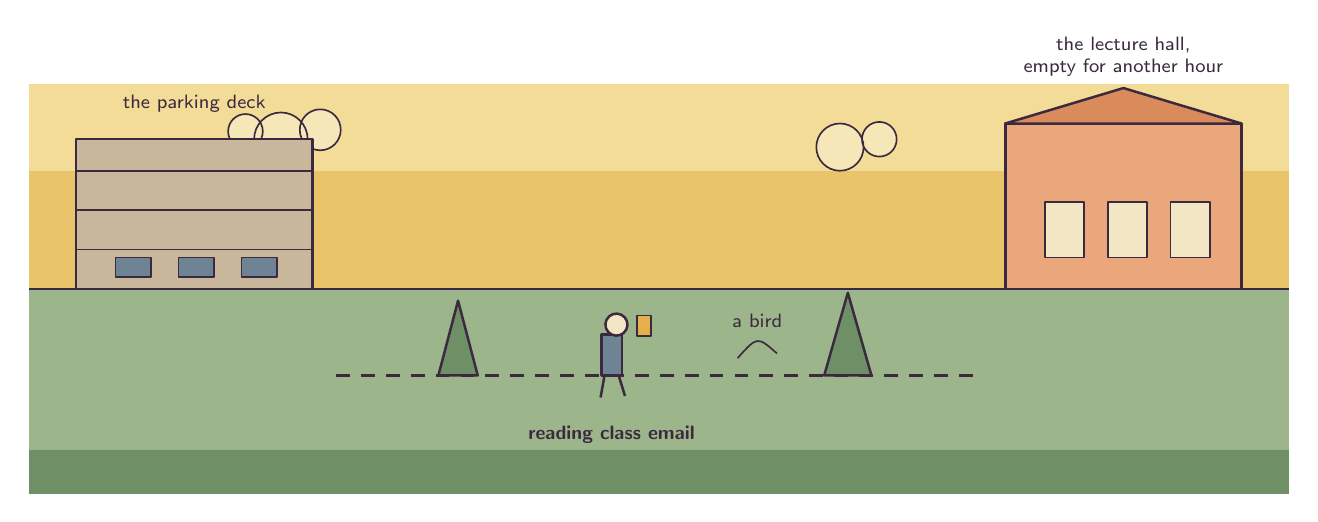
\begin{tikzpicture}[font=\sffamily]
  % Sky band, shared by every scene in this post.
  \fill[sky] (0,2.6) rectangle (16,5.2);
  \fill[skylight] (0,4.1) rectangle (16,5.2);
  \filldraw[fill=cloud, thinln] (3.2,4.5) circle (0.34) (3.7,4.62) circle (0.26) (2.75,4.6) circle (0.22);
  \filldraw[fill=cloud, thinln] (10.3,4.4) circle (0.3) (10.8,4.5) circle (0.22);
  % Ground.
  \fill[sage] (0,0) rectangle (16,2.6);
  \fill[sagedark] (0,0) rectangle (16,0.55);
  \draw[ln] (0,2.6) -- (16,2.6);
  % The parking deck, left.
  \filldraw[fill=stone, ln] (0.6,2.6) rectangle (3.6,4.5);
  \foreach \y in {3.1,3.6,4.1} \draw[thinln] (0.6,\y) -- (3.6,\y);
  \foreach \x in {1.1,1.9,2.7} \filldraw[fill=slate, thinln] (\x,2.75) rectangle (\x+0.45,3.0);
  \node[lab, text width=3cm] at (2.1,4.95) {the parking deck};
  % The lecture hall, right.
  \filldraw[fill=peach, ln] (12.4,2.6) rectangle (15.4,4.7);
  \filldraw[fill=peachdark, ln] (12.4,4.7) -- (13.9,5.15) -- (15.4,4.7) -- cycle;
  \foreach \x in {12.9,13.7,14.5} \filldraw[fill=cream, thinln] (\x,3.0) rectangle (\x+0.5,3.7);
  \node[lab, text width=3.4cm] at (13.9,5.55) {the lecture hall,\\empty for another hour};
  % The path, and the walker on it looking down.
  \draw[ln, dash pattern=on 5pt off 4pt] (3.9,1.5) -- (12.1,1.5);
  \walker{7.4}{1.5}{slate}{-26}
  \filldraw[fill=gold, thinln] (7.72,2.0) rectangle (7.9,2.26);
  \node[tag, text width=3.4cm] at (7.4,0.75) {reading class email};
  % What is actually around, unattended.
  \filldraw[fill=sagedark, ln] (5.2,1.5) -- (5.45,2.45) -- (5.7,1.5) -- cycle;
  \filldraw[fill=sagedark, ln] (10.1,1.5) -- (10.4,2.55) -- (10.7,1.5) -- cycle;
  \draw[thinln] (9.0,1.72) .. controls (9.25,2.0) .. (9.5,1.78);
  \node[lab] at (9.25,2.2) {a bird};
\end{tikzpicture}
\end{document}
